\documentclass[12pt]{article}
\usepackage[margin=1in]{geometry} %1 inch margins
\usepackage{verbatim} %multi-line comment
\usepackage{graphicx} %graphics
\usepackage{fancyhdr} %custom header
\usepackage{amsmath} %math
\usepackage{amssymb} %math symbols
\usepackage{bm} %bold math text
\usepackage{bbm} %indicators
\usepackage{soul} %for underlining
\usepackage{listings}
\usepackage{booktabs}
%\pagenumbering{gobble} %no page numberings
\pagestyle{fancy}
\newcommand{\indep}{\raisebox{0.05em}{\rotatebox[origin=c]{90}{$\models$}}}
\allowdisplaybreaks

\renewcommand{\headrulewidth}{0pt}
\lhead{CS 208 - Applied Privacy for Data Science\\Harvard University}
\rhead{Huang, Jason\\Homework 2}
%%%%%%%%%%% BEGIN DOCUMENT
\begin{document}
\begin{center}
	{\Large \textbf{CS 208 - Applied Privacy for Data Science}}\\
	{\Large \textbf{Homework 2}}\\
	\vspace*{0.1in}
	Jason Huang\\
	Spring 2019 - Harvard University\\
\end{center}

The public Github repo containing all work is at https://github.com/TurboFreeze/cs208hw. All code has also been included in the appendix of this PDF as specified.\\

{\large\textbf{Problem 1}}

\begin{enumerate}
	\item[(i)] \begin{enumerate}
	\item The clamping function is effectively applying a post-processing function to the noisy query result. In other words, Laplace noise is added to the true mean $\bar{x}$, which must be $(\epsilon, 0)$-DP. The following clamping function does not change the privacy characteristics guaranteed by differential privacy, meaning that this mechanism \textbf{meets the definition} of $(\epsilon, 0)$-DP (following directly by privacy under post-processing and the proof of Laplace DP).
	
	Note that the scale factor parameter of the Laplace distribution should be set to $s = GS_q/\epsilon$ for differential privacy, meaning that $\epsilon = GS_q/s$. In this case, the global sensitivity $GS_q$ is the maximum change that can be affected to the statistic by a single entry's change, which in this case would be $1/n$ for the mean. Furthermore $s = 2 / n$. The smallest $\epsilon$ for which this holds would then be $\epsilon = (1/n) / (2/n) \implies \boxed{\epsilon= 0.5}$.
	\item An $\epsilon$ was found in the previous part so no $\delta$ is needed.
	\item Again, this is effectively the standard Laplace mechanism, and as seen before, the differentially private mean with Laplace noise can be generalized by clamping at any domain $[a, b]$ with $\epsilon$ being generally defined as $\epsilon = GS_q / s = (b- a)/(2/n)=\boxed{n(b-a)/2}$.
	\end{enumerate}
	\item[(ii)] \begin{enumerate}
	\item The intuition here is that for noise in the interval $(-1, 1)$, the densities of the Laplacian noise have the proper ratio. Because of the clamping function, $P[M(x) = r]$ will only have nonzero probability within $[\bar{x}-1,\bar{x} + 1]$, but $P[M(x') = r]$ will be nonzero in $[\bar{x}'-1,\bar{x}' + 1]$. In other words, $\exists r \in [\bar{x}-1,\bar{x} + 1]$ s.t. $P[M(x') = r] = 0$, thereby showing that this algorithm \textbf{does not meet} the definition of $(\epsilon, 0)$-DP.
	%The intuition here is that for noise in the interval $(-1, 1)$, the densities of the Laplacian noise have the proper ratio. However, at the endpoints, because the noise is clipped to this interval, the ratios are no longer appropriate; in fact, it is effectively the ratio of cumulative densities at the endpoints rather than probability densities. Since it should be intuitively clear that the claims here hold for within the interval, only the endpoints (of the noise) will be investigated in greater detail.
	\item Derive $\delta$ as by noting that for two neighboring datasets $x, x'$ to yield the maximum possible lower bound for $\delta$, first set an $\epsilon = 0.5$ as was derived for mechanism 1. Recall that $M(x)$ is nonzero only in $[\bar{x}-1,\bar{x} + 1]$ and $M(x')$ only in $[\bar{x}'-1,\bar{x}' + 1]$. That means the difference in the below expression for $\delta$ will be zero except (assuming that $\bar{x}' > \bar{x}$) in $(\bar{x} - 1, \bar{x}' - 1]$.
	\begin{align*}
		\delta &\geq \underset{x\sim x'}{\text{max}}\left(\int_y\text{max}\left(P[M(x) \in y]-e^{\epsilon}P[M(x') =y], 0\right)\right)
	\end{align*}
	That means instead of integrating all $y$, simply focus on this interval where $P[M(x') =y]=0$, which would be in $(\bar{x} - 1, \bar{x}' - 1]$. Now:
	\begin{align*}
		\delta &\geq \underset{x\sim x'}{\text{max}}\left(\text{max}\left(P[M(x) \in (\bar{x} - 1, \bar{x}' - 1)]-e^{\epsilon}P[M(x') =(\bar{x} - 1, \bar{x}' - 1)], 0\right)\right)\\
		&= \underset{x\sim x'}{\text{max}}\left(\text{max}\left(P[M(x) \in (\bar{x} - 1, \bar{x}'- 1]]-e^{\epsilon}*0, 0\right)\right)\\
		&= \underset{x\sim x'}{\text{max}}\left(P[M(x) \in (\bar{x} - 1, \bar{x}'- 1]]\right)
	\end{align*}
	This is simply the probability that $M(x)$ is greater than $\bar{x}' + 1$, which can be found by the CDF of the Laplace distribution ($1-\text{exp}(-(x-\mu)/s)/2$ where $\mu = \bar{x}$ in this case because it is being added to the zero-mean Laplace and $s = 2/n$ Laplace noise scale parameter).
	\begin{align*}
	\delta &\geq P[M(x) \in (\bar{x} - 1, \bar{x}' - 1]]\\
	&= P[M(x) \leq \bar{x}' - 1]\\
	&= \dfrac{1}{2}\text{exp}\left(-\dfrac{ \bar{x}' - 1 - \bar{x}}{2/n}\right)\\
	&=  \dfrac{1}{2}\text{exp}\left(- \dfrac{n(\bar{x}' - 1 - \bar{x})}{2}\right)
	\end{align*}
	Finally here, $\bar{x}' - \bar{x} \geq 1/n$ as the global sensitivity, so find $\delta$ to be as follows:
	\begin{align*}
	\delta &\geq \dfrac{1}{2}\text{exp}\left(- \dfrac{n(\bar{x}' - 1 - \bar{x})}{2}\right)\\
	&\geq \dfrac{1}{2} \text{exp} \left(- \dfrac{n(1-1/n)}{2}\right)\\
	&= \dfrac{1}{2} \text{exp} \left(- \dfrac{n - 1}{2}\right)
	\end{align*}
	$\therefore$ The smallest $\delta$ would be $\boxed{\delta = \frac{1}{2} \text{exp} \left(- \frac{n - 1}{2}\right)}$ along with $\boxed{\epsilon = 0.5}$ as found for the first mechanism.
	\item Here the bounds for clamping are actually independent of the bounds of the data domain. Note that the $\delta$ arises (this is also a useful intuitive formulation for understanding how $\delta$ was derived in the previous part) from the $(\bar{x} - 1, \bar{x}' - 1]$, which is the interval that is covered by one noise but not the other, which is clearly independent of the data bounds. However, it is dependent on $n$ as formulated in the answer in the previous part $\boxed{\delta = \text{exp} (- (n - 1)/2)/2}$, while $\epsilon$ will now be converted to the general form as found for mechanism 1 to depend on $n$ with $\boxed{\epsilon = n(b-a)/2}$.
	\end{enumerate}
	\item[(iii)] 
	\begin{enumerate}
	\item Since the mechanism release value is binary, the upper bound of the ratio of probabilities can be considered as simply the maximum of either the $r=0$ or $r=1$. Again consider neighboring datasets $x$ and $x'$.
	\begin{align*}
		\dfrac{P[M(x') = r]}{P[M(x)=r]} &\leq \text{max}\left(\dfrac{P[M(x') = 0]}{P[M(x)=0]}, \dfrac{P[M(x') = 1]}{P[M(x)=1]}\right)\\
		&= \text{max}\left(\dfrac{1-\bar{x}'}{1-\bar{x}}, \dfrac{\bar{x}'}{\bar{x}}\right)\\
		&= \text{max}\left(\dfrac{1-\bar{x}'}{1-\bar{x}} - \dfrac{1-\bar{x}}{1-\bar{x}} + \dfrac{1-\bar{x}}{1-\bar{x}} , \dfrac{\bar{x}'}{\bar{x}} - \dfrac{\bar{x}}{\bar{x}} + \dfrac{\bar{x}}{\bar{x}}\right)\\
		&= \text{max}\left(\dfrac{\bar{x}-\bar{x}'}{1-\bar{x}} + 1, \dfrac{\bar{x}'-\bar{x}}{\bar{x}} + 1\right)\\
		&= \text{max}\left(\dfrac{\bar{x}-\bar{x}'}{1-\bar{x}}, \dfrac{\bar{x}'-\bar{x}}{\bar{x}}\right)+1
	\end{align*}
	Since these means can be as close to 0 or 1 as possible, and there are means in the denominator, that means this max can be potentially infinitely large and as a result this mechanism \textbf{does not satisfy} $(\epsilon, 0)$-DP.
	\item Calculating this over the entire space of $y$ simply consists of a sum for the cases of when $y=0$ and $y=1$, as follows.
	\begin{align*}
		\delta &\geq \underset{x\sim x'}{\text{max}}\left(\int_y \text{max}\left(P[M(x) = y]-e^{\epsilon}P[M(x')=y], 0\right)\right)\\
		&= \underset{x\sim x'}{\text{max}}(\text{max}\left(P[M(x) = 1]-e^{\epsilon}P[M(x')=1], 0\right)\\ &\qquad+ \text{max}\left(P[M(x) = 0]-e^{\epsilon}P[M(x')=0], 0\right))\\
		&\geq (\bar{x} - \bar{x}') + (1-\bar{x} - (1-\bar{x}'))\\
		&\geq \bar{x} - \bar{x}'\\
		&= GS\\
		&= \dfrac{1}{n}
	\end{align*}
	The smallest $\delta$ for which this would work would be $\boxed{\delta = 1/n}$ along with a finite $\epsilon$ of 0.
	\item Instead of releasing 1 and 0, release the upper bound $b$ with probability $\bar{x}$ and the lower bound $a$ with probability $1-\bar{x}$, with everything else remaining the same. As noted earlier, no $\epsilon$ is needed, so it can remain 0. The $\delta$ needed would simply be updated to be $1/n$ as previously found to get $\boxed{\epsilon=0, \delta=1/n}$ in the general case.
	\end{enumerate}
	\item[(iv)] \begin{enumerate}
	\item For the mean of a neighboring data set $\bar{x}'$, let a corresponding $Y'$ refer to the probability density function with $\bar{x}'$. The ratio of probabilities is then simply the ratio of the PDFs. Also outside of $[0, 1]$, any $\epsilon$ is valid because the probabilities (based on the density function case) is 0 for both.
	\begin{align*}
		\dfrac{P[M(x') = r]}{P[M(x)=r]} &= \dfrac{f_{Y'}(y)}{f_Y(y)}\\
		&= \dfrac{\frac{e^{-n|y-\bar{x}'|/10}}{\int_0^1 e^{-n|z-\bar{x}'|/10} dz}}{\frac{e^{-n|y-\bar{x}|/10}}{\int_0^1 e^{-n|z-\bar{x}|/10} dz}}\\
		&= \dfrac{e^{-n|y-\bar{x}'|/10}}{\int_0^1 e^{-n|z-\bar{x}'|/10} dz}\dfrac{\int_0^1 e^{-n|z-\bar{x}|/10} dz}{e^{-n|y-\bar{x}|/10}}\\
		&= \dfrac{\int_0^1 e^{-n|z-\bar{x}|/10} dz}{\int_0^1 e^{-n|z-\bar{x}'|/10} dz}\dfrac{e^{-n|y-\bar{x}'|/10}}{e^{-n|y-\bar{x}|/10}}\\
		&= \dfrac{\int_0^1 e^{-n|z-\bar{x}|/10} dz}{\int_0^1 e^{-n|z-\bar{x}'|/10} dz}e^{-n(|y-\bar{x}'|+|y-\bar{x}|)/10}\\
		&\leq \dfrac{\int_0^1 e^{-n|z-\bar{x}|/10} dz}{\int_0^1 e^{-n|z-\bar{x}'|/10} dz}e^{-n|\bar{x}'-\bar{x}|/10}
	\end{align*}
	\begin{comment}%%%%%
	The triangle inequality was used to introduce the inequality and will be shortly used again. Now since the later ratio is a constant with respect to the integrals, it can be moved into the upper integral with the triangle inequality again.
	\begin{align*}
		\dfrac{P[M(x') = r]}{P[M(x)=r]} &\leq \dfrac{\int_0^1 e^{-n|z-\bar{x}|/10} dz}{\int_0^1 e^{-n|z-\bar{x}'|/10} dz}e^{-n|\bar{x}'-\bar{x}|/10}\\
		&= \dfrac{\int_0^1 e^{-n|z-\bar{x}|/10-n|\bar{x}'-\bar{x}|/10} dz}{\int_0^1 e^{-n|z-\bar{x}'|/10} dz}\\
		&= \dfrac{\int_0^1 e^{-n(|z-\bar{x}|+|\bar{x}'-\bar{x}|)/10} dz}{\int_0^1 e^{-n|z-\bar{x}'|/10} dz}\\
		&\leq \dfrac{\int_0^1 e^{-n|z-\bar{x}'|/10} dz}{\int_0^1 e^{-n|z-\bar{x}'|/10} dz}\\
		&=1
	\end{align*}
	\end{comment}
	Make the observation that $|e^{-n|z-\bar{x}|/10}| \leq e^{-n|z-\bar{x}'|/10-n(1/n)/10} =e^{-n|z-\bar{x}'|/10}e^{-1/10}$ and also $|\bar{x}'-\bar{x}| \leq GS = 1/n$.
	\begin{align*}
		\dfrac{P[M(x') = r]}{P[M(x)=r]} &\leq \dfrac{\int_0^1 e^{-n|z-\bar{x}|/10} dz}{\int_0^1 e^{-n|z-\bar{x}'|/10} dz}e^{-n|\bar{x}'-\bar{x}|/10}\\
		&\leq \dfrac{\int_0^1 e^{-n|z-\bar{x}'|/10}e^{-1/10} dz}{\int_0^1 e^{-n|z-\bar{x}'|/10} dz}e^{-n(1/n)/10}\\
		&= \dfrac{\int_0^1 e^{-n|z-\bar{x}'|/10}dz}{\int_0^1 e^{-n|z-\bar{x}'|/10} dz}e^{-1/10} e^{-1/10}\\
		&=e^{1/5}
	\end{align*}
	This algorithm therefore \textbf{meets the definition} of $(\epsilon, 0)$-DP with $\boxed{\epsilon=0.2}$.
	\item Since $(\epsilon, 0)$-DP is satisfied, the smallest value of $\delta$ needed is 0.
	\item The only thing that would really change dependent on either $n$ or the new bounds $[a, b]$ would be the bounds of integration. The $\epsilon$ value is independent of either value and can be anything greater than or equal to what was found in the previous part, while no $\delta$ is needed.
	\end{enumerate}
\end{enumerate}
(d) The first algorithm appears to be the best for releasing a mean because it provides $(\epsilon, 0)$-DP unlike the chance of catastrophic failure introduced by $(\epsilon, \delta)$-DP in other algorithms. Note that neither is objectively better, just a design decision, but pure $\epsilon$ is the traditional definition that is easier to work with and preferred here. At the same time, the first algorithm still provides meaningful results with high utility; the third algorithm, for example, will always release only 0 or 1, which provides very little utility in the released statistic.

\pagebreak

{\large\textbf{Problem 2}}

\textbf{(a)} The DGP is the following likelihood of some data vector $k\in\mathbb{N}^n$:
\[P(\mathbf{x} = \mathbf{k}) = \prod\limits^n_{i=1} \dfrac{10^{\mathbf{k}_i}e^{-10}}{\mathbf{k}_i!}\]
The DGP function was implemented using a Poisson random draw.

\emph{See the attached R script \texttt{q2.R} for the implementation}.\\

\textbf{(b)} The first mechanism was chosen, involving clamping after Laplace noise has been added.

\emph{See the attached R script \texttt{q2.R} for the implementation}.\\

\textbf{(c)} The optimal value $b^*$ for $b$ is $\boxed{b^* \approx 15}$. As expected, root mean squared error is indeed high with small clamping regions and decreases as it becomes more appropriate, with large clamping regions yielding high RMSE again.

\begin{center}
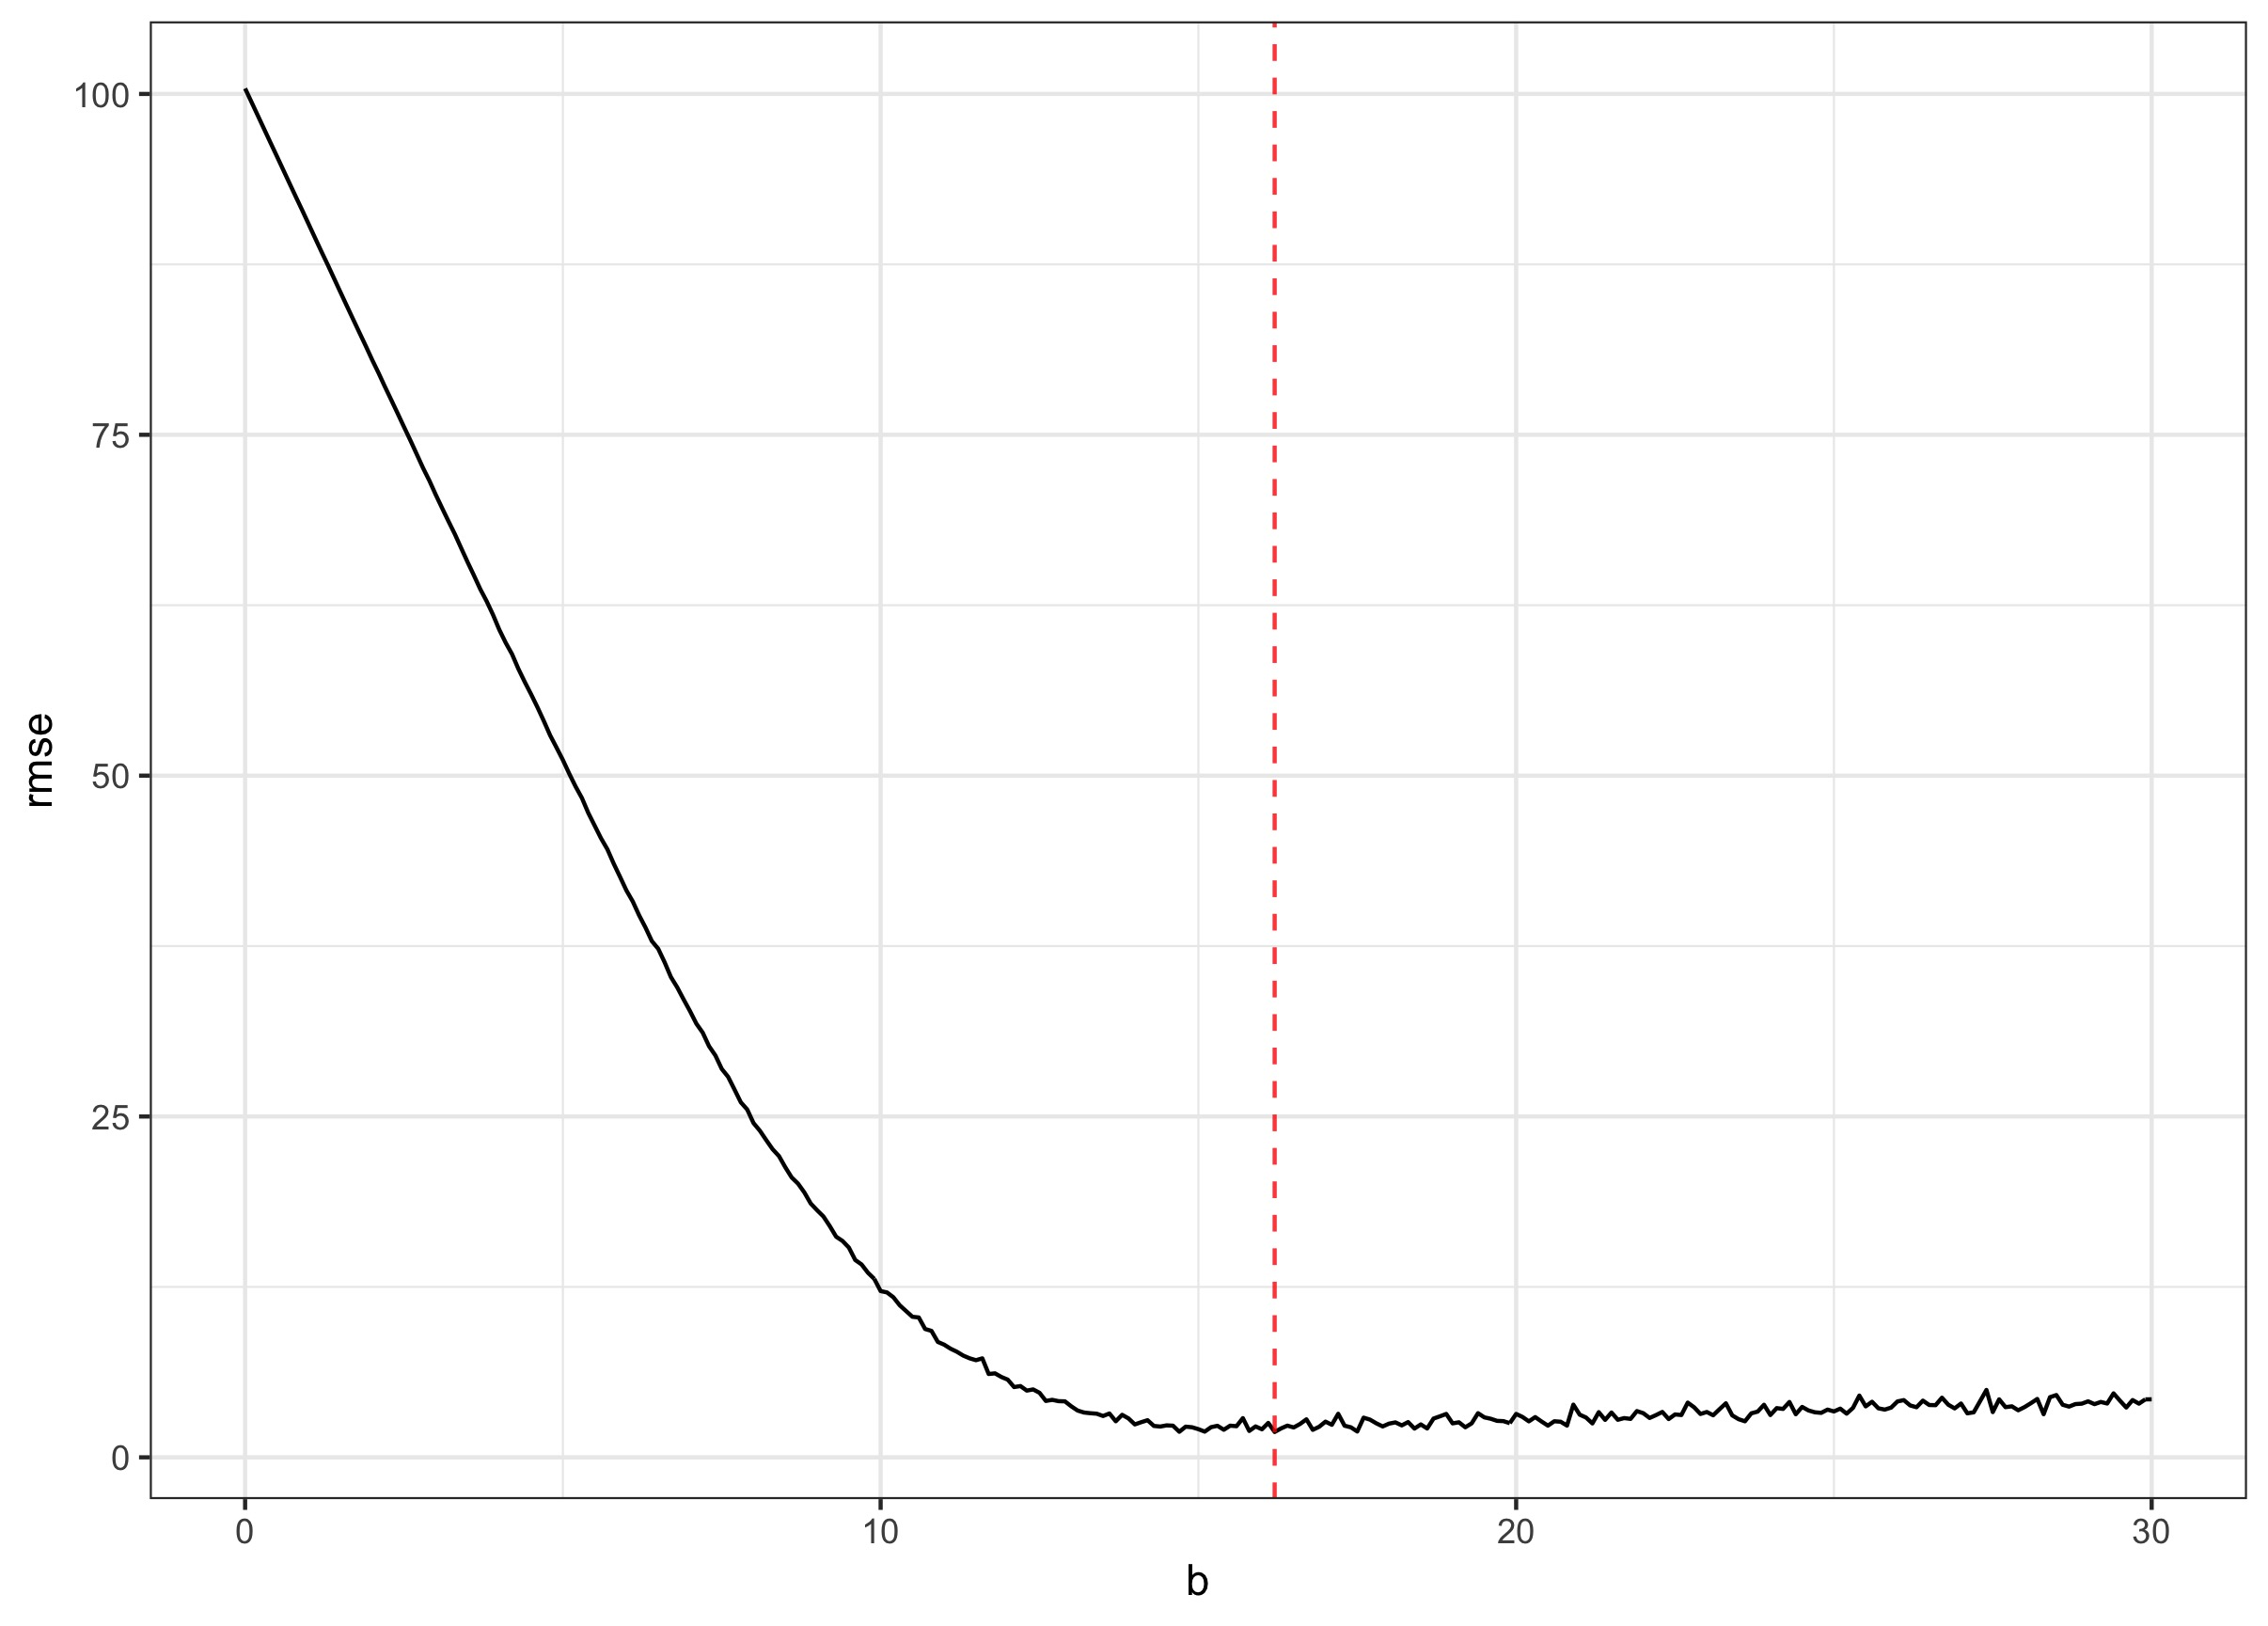
\includegraphics[width=0.7\textwidth]{clamping}
\end{center}

\emph{See the attached R script \texttt{q2.R} for the implementation}.\\

\textbf{(d)} This approach is not safe and might violate differential privacy because it implicitly incorporates information about the dataset that is not included in the data. More specifically, bootstrapping is powerful because of its very ability to simulate the data generating process and the distribution of the data. Therefore, bootstrapping to find an estimate for the optimal value $b^*$ is effectively the same thing as calculating the true optimal $b^*$, only numerically instead of analytically. Now, knowing the optimal $b^*$ violates privacy because it also provides insight into the distribution (i.e. one of the ways this can be intuitively described is as an approximate maximum of everything that is not an outlier). This is similar to the idea of why local sensitivity, which is a characteristic of the data set, is not $(\epsilon, \delta)$-DP but global sensitivity is. The optimal $b^*$ is a specific data-dependent attribute of the data set that can leak privacy if not controlled for, as is the case with bootstrapping here.\\

\textbf{(e)} Use an external reference for determining an approximation for $b^*$. Generally, a similar public data set (i.e. past iterations of the census or different geographic tracts that have been made public) can help provide a rough estimate of the upper bound for the individual. Often times, a reasonable heuristic can be used based on common knowledge, such as the rough range of human ages or other metadata provided for the data set (i.e. in a codebook or schema).\\

\pagebreak

{\large\textbf{Problem 3}}

\textbf{(a)} There are differentially private techniques to release the means $\bar{y}$ and $\bar{x}$ as well as the slope $\hat{\beta}$. However, given the careful considerations needed for the slope $\hat{\beta}$, it may be challenging to come up with a single differentially private mechanism to derive the intercept estimate. However $\hat{\alpha} = \bar{y} - \hat{\beta}\bar{x}$ lends itself nicely to privacy preservation under composition and post-processing. Since there are three differentially private statistics needed here of $\bar{x}, \bar{y}, \hat{\beta}$, for a total epsilon budget of $\epsilon_t$, then calculate differentially private releases of each statistic with $\epsilon = \epsilon_t/4$ (note that the slope $\hat{\beta}$ is actually two statistics of covariance and variance in the numerator and denominator respectively) to yield $(\epsilon_t / 4,0)$-DP statistics. Since post-processing is allowed without affecting privacy, then this three differentially private statistics will lead to $\epsilon_t / 4 + \epsilon_t / 4 + \epsilon_t / 2 = \epsilon_t$ differential privacy for $\hat{\alpha}$ by composition and $\epsilon_t/4 + \epsilon_t/4 = \epsilon_t/2$ differential privacy for $\hat{\beta}$ (which is used in $\hat{\alpha}$ and does not require separate consumption of the budget). Therefore, the overall method for computing both $\hat{\alpha}$ and $\hat{\beta}$ would be $\epsilon_t$-DP, as desired.

Since the data $x_i$ is generated by a Poisson process according to the previous problem, it can be clamped using the optimal value of $b^*\approx 10$ found before. Since there is a linear relationship between $x_i$ and $y_i$ here (and it is known in the following part that the slope is simply 1), then similarly clamp $y_i$ by $b^* \approx 15$.

\emph{See the attached R script \texttt{q3.R} for the implementation}.\\

\textbf{(b)} A Monte Carlo simulation yields the following plots. The differentially private regression is in red while the non-private simple linear regression results are in green. Here is the traceplot and scatter plot of mean squared residuals against the number of simulations $n$. Note also that the residual error is clipped to (0, 10), with a very small number of differentially private errors (around 25 out of 1000) jumping well beyond the upper bound of 10.
\begin{center}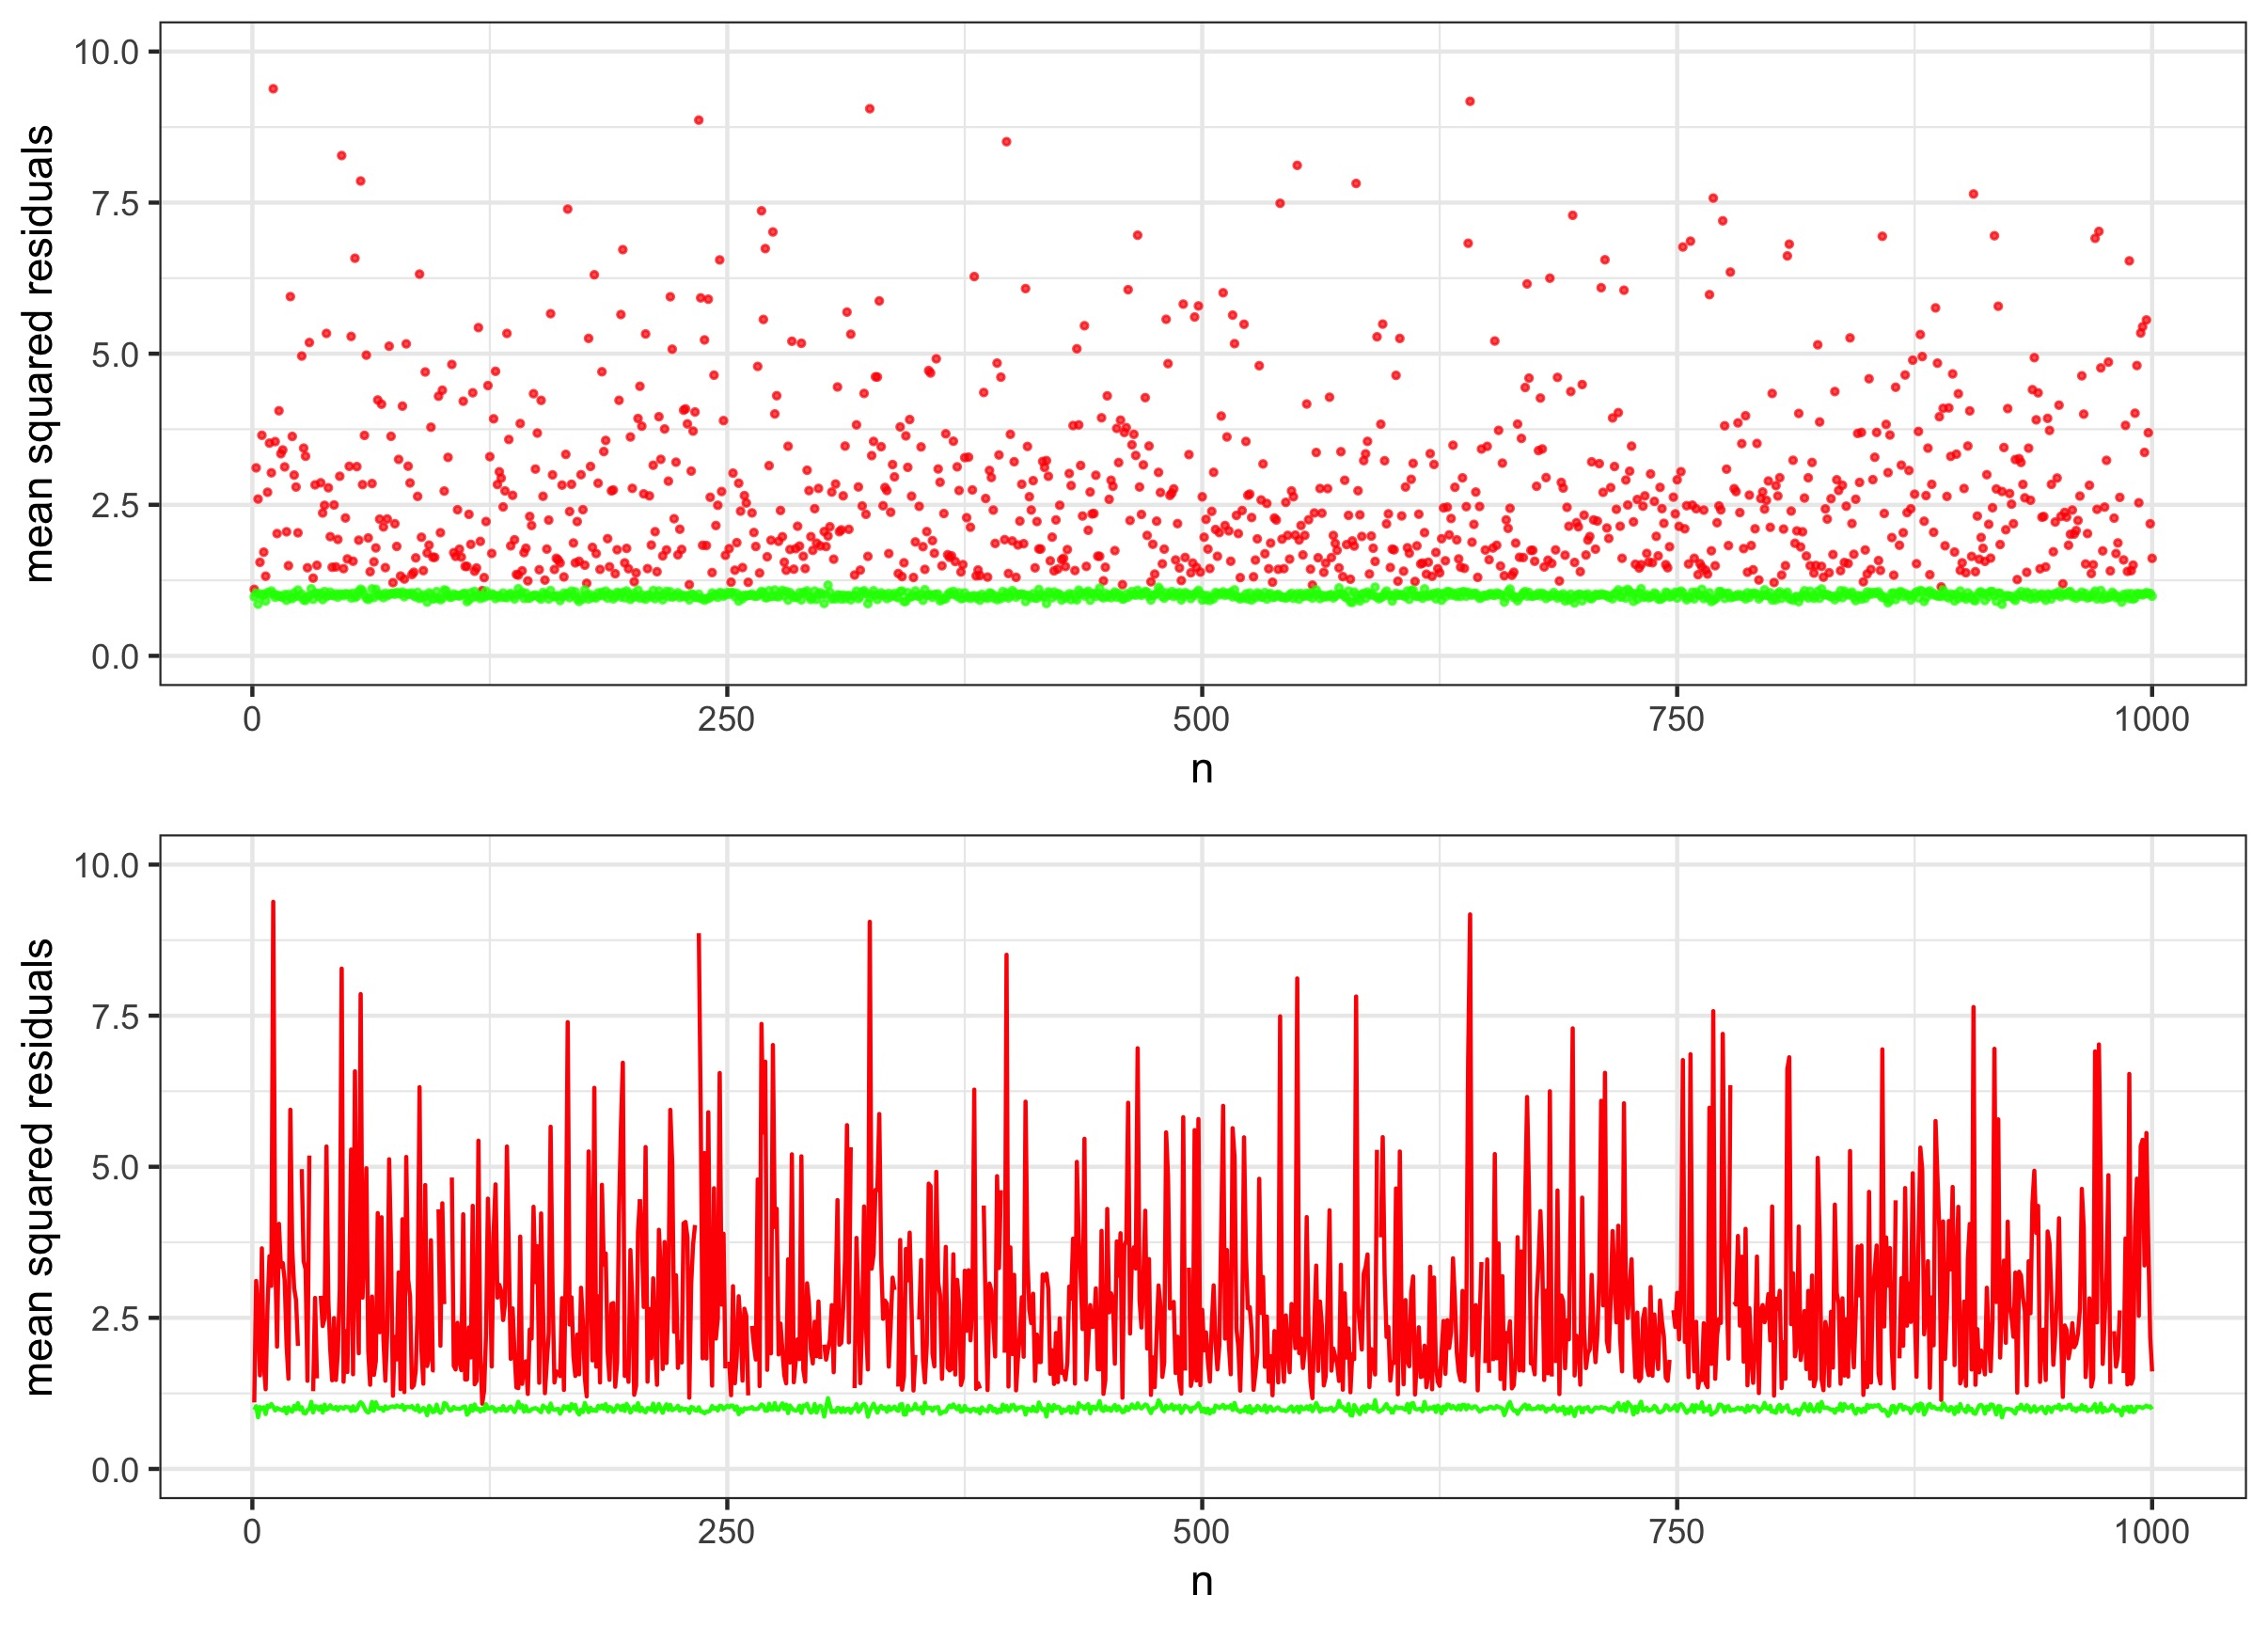
\includegraphics[width=0.75\textwidth]{msrs}\end{center}
When examining the distribution of mean-squared residuals as desired, then following density curves were calculated.
\begin{center}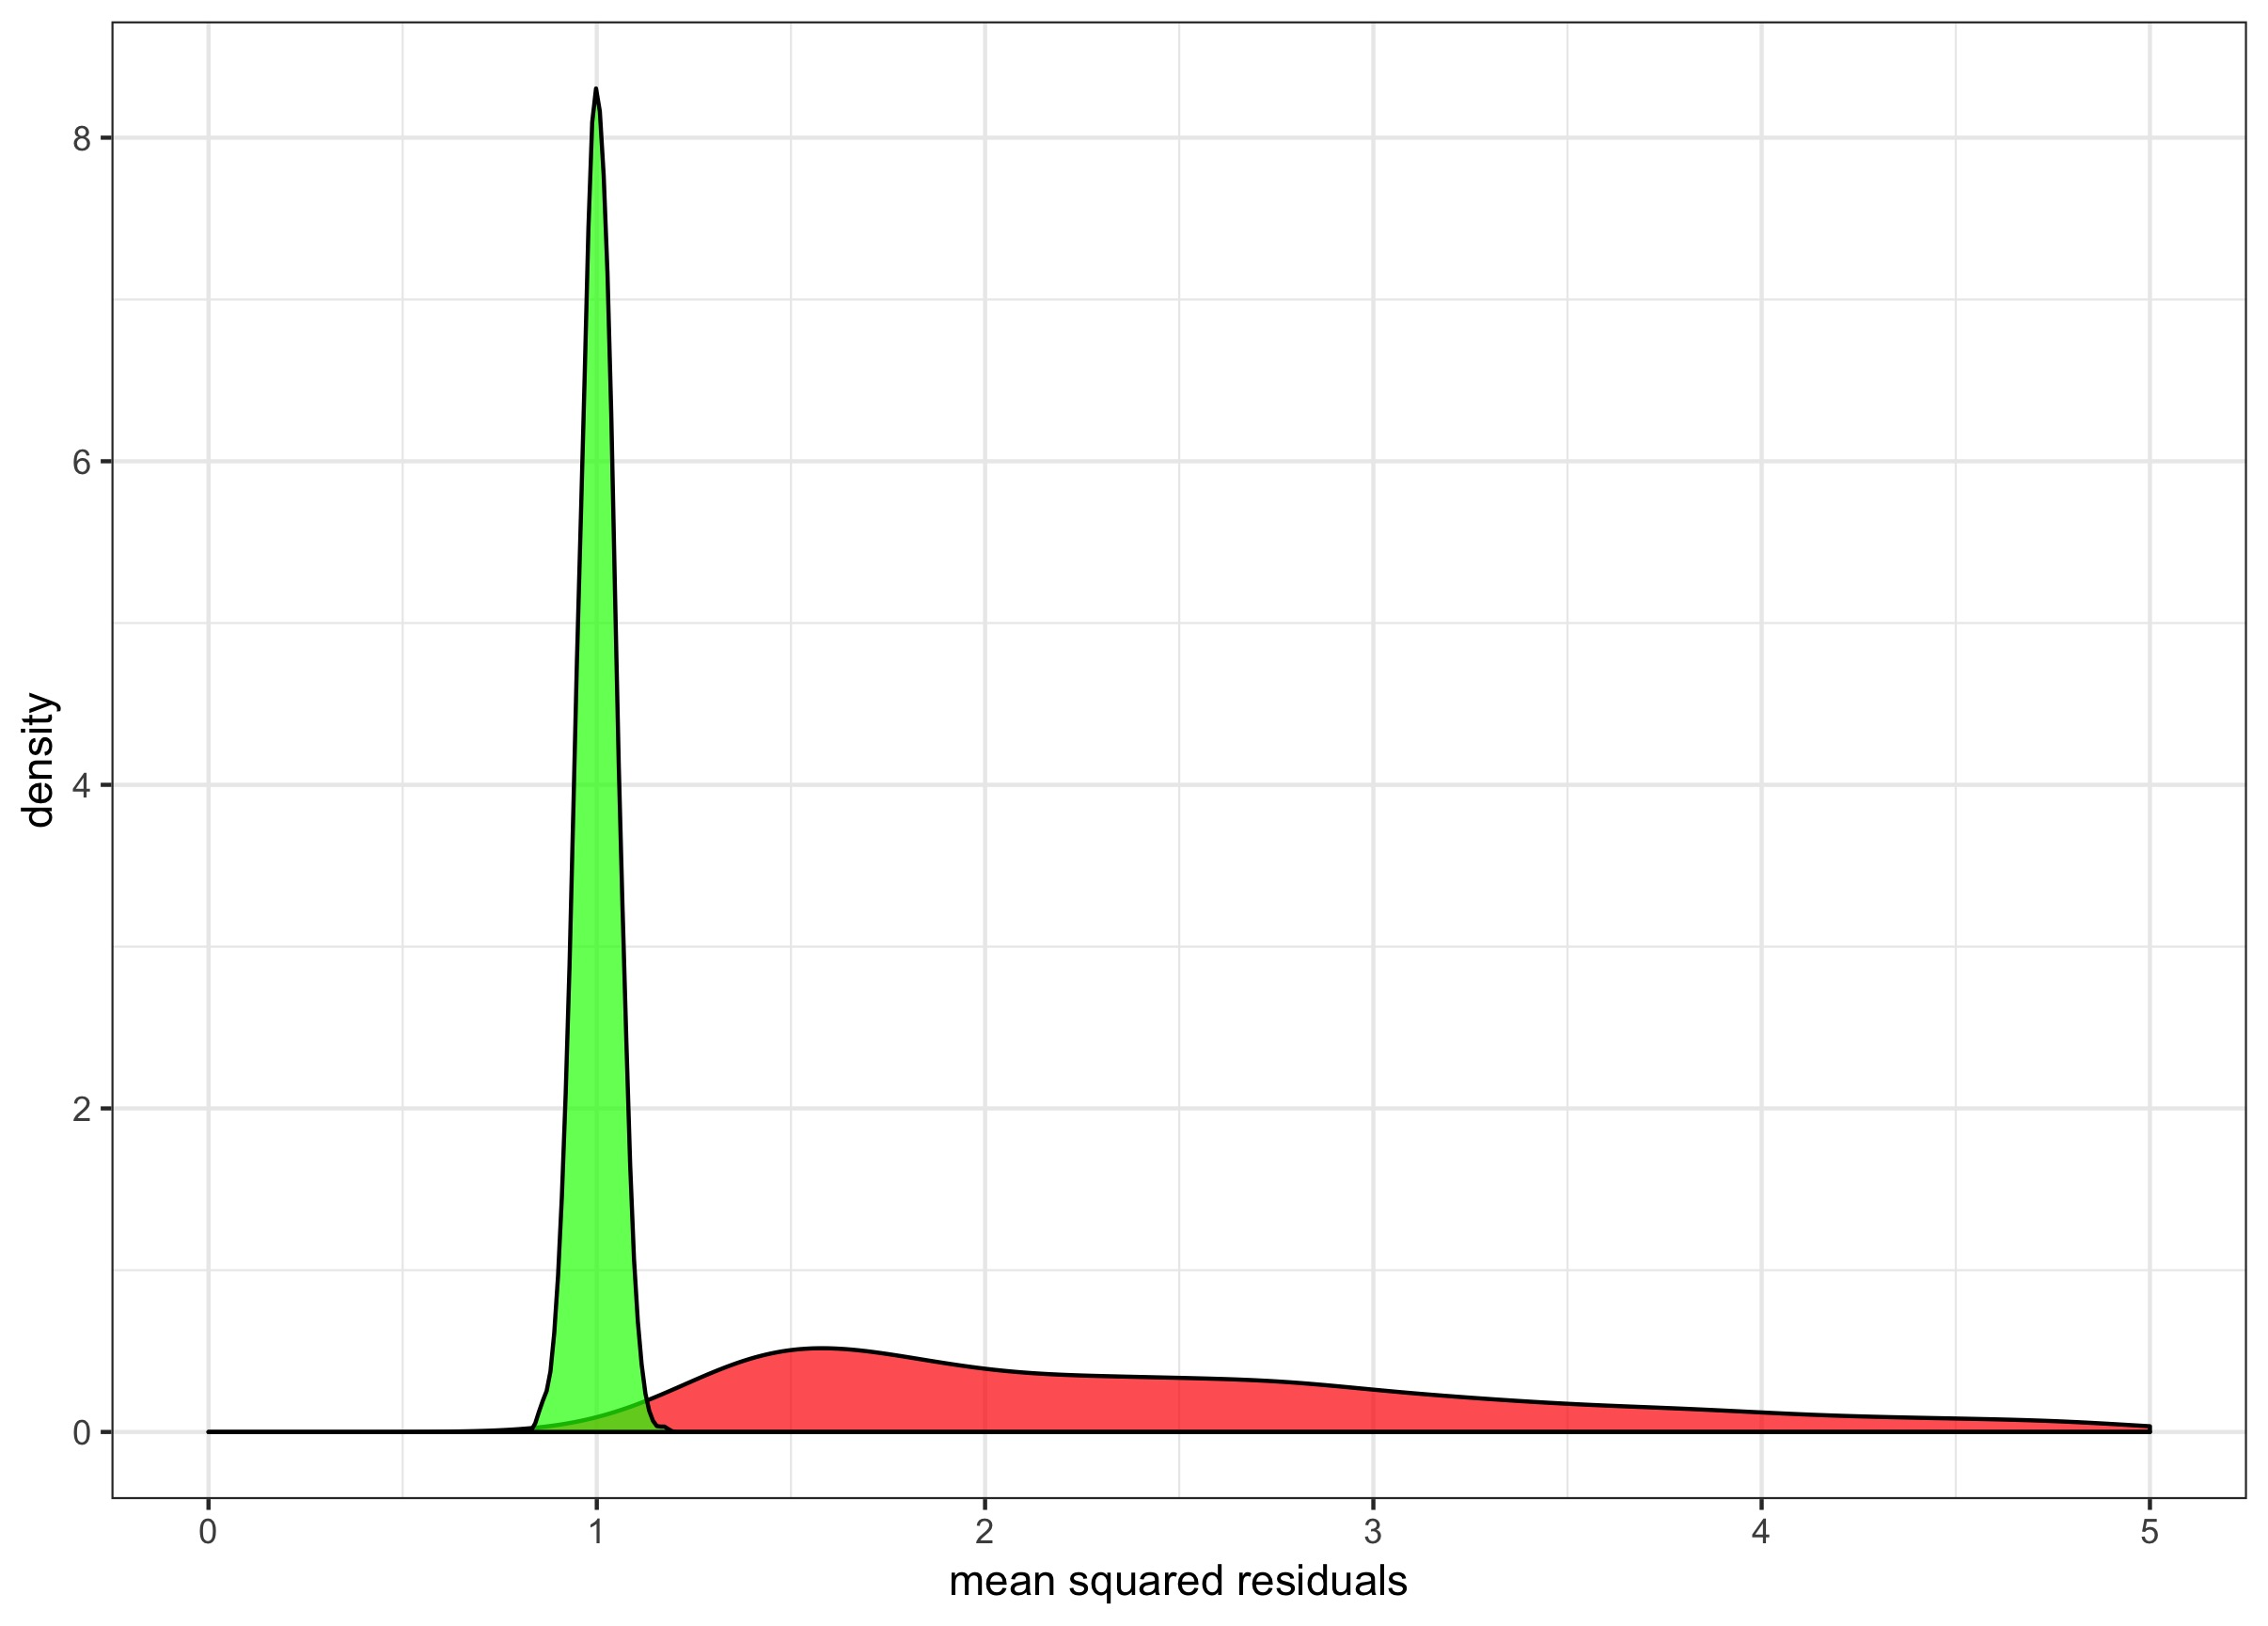
\includegraphics[width=0.75\textwidth]{msrsdist}\end{center} 
Recall that mean squared residuals is a measure for residuals, or the addition of noise on top of everything that is not already explained by the model. It can be seen from the above graphic that the non-private residuals in green peak tightly around 1, likely due to the fact that the noise added is Gaussian with standard deviation of 1. In fact, the distribution of the noise itself is symmetrical around 1 and \emph{appears Gaussian in distribution}. Similarly, the differentially private residuals in red have a mode in density between 1 and 2, and has a substantially longer right tail. In fact, the entire distribution is reminiscent of the \emph{Poisson distribution}, even specifically Poisson process with $\lambda=10$, speaking to the ability of this differentially private mechanism to inject noise while accurately reflecting the behavior of the true data generating process.

\emph{See the attached R script \texttt{q3.R} for the implementation}.\\

\textbf{(c)} Grid search was implemented here by setting a hyperparameter domain of $x_1, x_2, x_3, x_4 \in \mathcal{D} = \{0.1, 0.2, \dots, 1\}$, recursively creating every possible combination of 4 values from this domain and most importantly, normalizing these to create a distribution; in other words, such that the normalized vector $\mathbf{x}' = (x_1', x_2', x_3', x_4')$ has $\sum_{i=1}^4x'_i = 1$. This is the process by which the $|\mathcal{D}^4| = 10000$ combinations within the parameter space are generated and calculated.

The differentially private regression was run on each of these parameter spaces, with the mean squared residuals calculated. With equal partitioning of $\epsilon$, the mean squared residuals is $\approx 6.070752$. With the 10000 combinations tested by the grid search, the top 10 with lowest mean squared residual error were found, with the corresponding hyperparameter configuration included all in the table below. The mean and median of these best 10 configurations is also included as a rough approximation of the optimal configuration for distribution $\epsilon$. Note that these do have substantially lower mean squared residuals than an equal partition.

\begin{center}
\begin{tabular}{|c||c|c|c|c||c|}\hline
	& $\epsilon$ for $\text{Cov}(x, y)$ & $\epsilon$ for $\text{Var}(x)$ &  $\epsilon$ for $\bar{x}$ & $\epsilon$ for $\bar{y}$ & Error\\\hline\hline
	Even partition & 0.25 & 0.25 & 0.25 & 0.25 & 6.070752 \\\hline\hline
	&0.18750000 & 0.56250000&0.06250000&0.18750000& 0.9590050 \\
	 & 0.40000000 & 0.40000000 & 0.06666667 & 0.13333333 & 0.9595579 \\
	 & 0.05555556 & 0.33333333 & 0.55555556 & 0.05555556 & 0.9906817 \\
	 & 0.15384615 & 0.07692308 & 0.23076923 & 0.53846154 & 1.0065410 \\
	 & 0.30434783 & 0.34782609 & 0.04347826 & 0.30434783 & 1.0109240 \\
	 & 0.33333333 & 0.26666667 & 0.26666667 & 0.13333333 & 1.0116808 \\
	 & 0.28571429 & 0.42857143 & 0.14285714 & 0.14285714 & 1.0236383 \\
	 & 0.40000000 & 0.24000000 & 0.04000000 & 0.32000000 & 1.0285891 \\
	 & 0.34782609 & 0.21739130 & 0.34782609 & 0.08695652 & 1.0321955 \\
	 & 0.37500000 & 0.37500000 & 0.08333333 & 0.16666667 & 1.0404765 \\\hline\hline
	 Mean&0.2843123 & 0.3248212 & 0.1839653 & 0.2069012 & \\
	 Median & 0.3188406 & 0.3405797 & 0.1130952 & 0.1547619 & \\\hline
\end{tabular}
\end{center}
There is a quite some variation among these best trials simply due to noise, hence taking the mean and median. There are nonetheless some patterns that are present, which the mean and median are particularly helpful in capturing, particularly the higher emphasis on $\text{Var}(x)$ and $\text{Cov}(x, y)$, and then the remaining $25\%-40\%$ for $\bar{y}$ and $\bar{x}$, in that order of decreasing weight.


\emph{See the attached R script \texttt{q3.R} for the implementation}.\\

\pagebreak

{\large\textbf{Problem 4}}

Use linearity of expectations and fundamental bridge to convert between probabilities and expectation of indicators.
\begin{align*}
	\mathbb{E}[\#\{ i\in [n]: A(M(X))_i = X_i\} / n] &= \mathbb{E}[\mathbbm{1}\{ i\in [n]: A(M(X))_i = X_i\} / n]\\
	&= \mathbb{E}[\sum\limits^n_{i=1}\mathbbm{1}(A(M(X))_i = X_i) / n]\\
	&= \dfrac{1}{n}\sum\limits^n_{i=1}\mathbb{E}[\mathbbm{1}(A(M(X))_i = X_i)]\\
	&= \dfrac{1}{n}\sum\limits^n_{i=1}P(A(M(X))_i = X_i)\\
	&= P(A(M(X))_i = X_i)
\end{align*}
Where the last simplification is made by noting the independence of the $X_i$ data draws. Let there be a dataset $X^{i0}$ or $X^{i1}$ such that the $i^{th}$ row is changed to 0 or 1 respectively, with corresponding probabilities of $p$ and $1-p$ by the nature of the given Bernoulli data generating process. Now by the definition of $(\epsilon, \delta)$-DP:
\begin{align*}
	\mathbb{E}[\#\{ i\in [n]: A(M(X))_i = X_i\} / n] &= P(A(M(X))_i = X_i)\\
	&\leq e^{\epsilon}\cdot \text{max}\{P(A(M(X^{i0}))_i = X_i),P(A(M(X^{i1}))_i = X_i)\} + \delta\\
	&\leq e^{\epsilon}\cdot \text{max}\{p, 1-p\} + \delta
\end{align*}
The desired result has been shown.
\[\therefore\boxed{\mathbb{E}[\#\{ i\in [n]: A(M(X))_i = X_i\} / n] \leq e^{\epsilon} \cdot \text{max}\{p, 1-p\} + \delta}\text{ as desired}\]



\pagebreak

{\large\textbf{Problem 5}}

See final project next steps in separate file.

\pagebreak

{\large\textbf{Appendix}}

\textbf{Code for Problem 2}

\begin{lstlisting}[language=R]
##
## q2.r
##
## Evaluating DP algorithms with synthetic data
##
## JH 2019/03/10
##



##3 PART (A)
# data generating process
dgp <- function (n, lambda=10) {
  rpois(n, lambda)
}



### PART (B)

# sign function
sgn <- function(x) {
  return(ifelse(x < 0, -1, 1))
}

# laplace random draws
rlap <- function(mu=0, s=1, size=1) {
  p <- runif(size) - 0.5
  draws <- mu - s * sgn(p) * log(1 - 2 * abs(p))
  draws
}

# clamping helper function
clamp <- function (data, a, b) {
  data.clamped <- data
  data.clamped[data < a] <- a
  data.clamped[data > b] <- b
  data.clamped
}

# differentially private mechanism (clamping)
dpclamping <- function (data, epsilon, a=0, b) {
  mean.actual <- mean(clamp(data, a, b))
  
  # generate noise by Laplace mechanism
  data.len <- length(data)
  sensitivity <- (b - a) / data.len
  laplace.shift <- sensitivity / epsilon
  noise <- rlap(s=laplace.shift, size=1)
  
  # inject noise
  mean.noisy <- mean.actual + noise
  
  # apply clamping
  mean.clamped <- clamp(mean.noisy, a, b)
}



### PART (C)

# parameters
n <- 200
epsilon <- 0.5
b.seq <- seq(0, 30, by=0.1)
b.num <- length(b.seq)

# generate data
data.poisson <- dgp(n, lambda=10)

# calculate RMSE
rmse <- function (data, m) {
  sqrt(sum((data - m)^2))
}

n.trials <- 100
rmses <- vector("numeric", b.num)
for (i in 1:b.num) {
  
  dpmeans <- vector("numeric", n.trials)
  for (j in 1:n.trials) {
    # calculate dp query of mean
    dpmeans[j] <- dpclamping(data=data.poisson, epsilon=epsilon, b=b.seq[i])
  }
  # calculate and store RMSE
  rmses[i] <- rmse(dpmeans, m=mean(data.poisson))
}


# find index of minimum RMSE (optimal value of b)
b.optimal <- b.seq[which.min(rmses)]; b.optimal

#plot(b.seq, rmses, type='l') # uncomment if no ggplot

# visualize
rmsedata <- data.frame(b=b.seq, rmse=rmses)
library(ggplot2)
clamping.plot <- ggplot(rmsedata, aes(x=b, y=rmse)) +
  geom_line() +
  geom_vline(xintercept=b.optimal, color="red", alpha=0.8, linetype="dashed") +
  theme_bw()
clamping.plot
ggsave("clamping.jpg", clamping.plot)
\end{lstlisting}


\pagebreak

\textbf{Code for Problem 3}

\begin{lstlisting}[language=R]
##
## q3regression.r
##
## Differentially private regression
##
## JH 2019/03/10
##



### PART (A)

# optimal upper bound found in previous part
b.optimal <- 15

# data generating process
dgp <- function (n, lambda=10) {
  rpois(n, lambda)
}

# sign function
sgn <- function(x) {
  return(ifelse(x < 0, -1, 1))
}

# clamping helper function
clamp <- function (data, a, b) {
  data.clamped <- data
  data.clamped[data < a] <- a
  data.clamped[data > b] <- b
  data.clamped
}

# laplace random draws
rlap <- function(mu=0, s=1, size=1) {
  p <- runif(size) - 0.5
  draws <- mu - s * sgn(p) * log(1 - 2 * abs(p))
  draws
}

# differentially private mean release
dpmean <- function (data, epsilon, a=0, b) {
  mean.actual <- mean(clamp(data, a, b))
  
  # generate noise by Laplace mechanism
  data.len <- length(data)
  sensitivity <- (b - a) / data.len
  laplace.shift <- sensitivity / epsilon
  noise <- rlap(s=laplace.shift, size=1)
  
  # inject noise
  mean.noisy <- mean.actual + noise
  
  # apply clamping
  mean.clamped <- clamp(mean.noisy, a, b)
}


# Differentially private regression slope release (from provided code)
dpslope <- function (y, x, ylower=0, yupper=b.optimal, xlower=0, xupper=b.optimal, eps1, eps2){
  x <- clamp(x, xlower, xupper)
  y <- clamp(y, ylower, yupper)
  
  n <- length(x)
  sens.sxy <- (xupper - xlower) * (yupper - ylower)
  sens.sxx  <- (xupper - xlower)^2
  
  scale.sxy <- sens.sxy / eps1
  scale.sxx <- sens.sxx / eps2
  
  sensitive.value <- sum((x - mean(x)) * (y - mean(y))) / sum((x - mean(x))^2) 
  
  release.sxy <- sum((x - mean(x)) * (y - mean(y))) + rlap(mu=0, s=scale.sxy, size=1)
  release.sxx <- sum((x - mean(x))^2) + rlap(mu=0, s=scale.sxx, size=1)
  
  postprocess.beta <- release.sxy / release.sxx
  postprocess.beta
}

# Differentially private linear regression release of intercept and slope
dpregression <- function (y, x, ylower=0, yupper=b.optimal, xlower=0, xupper=b.optimal,
                          epsilon, epsilon.partition=c(0.25, 0.25, 0.25, 0.25)) {
  x <- clamp(x, xlower, xupper)
  y <- clamp(y, ylower, yupper)
  
  # calculate dp slope
  dpbeta <- dpslope(y, x, ylower, yupper, xlower, xupper,
                    epsilon * epsilon.partition[1], epsilon * epsilon.partition[2])
  
  # calculate dp intercept
  dpmean.x <- dpmean(x, epsilon * epsilon.partition[3], b=xupper)
  dpmean.y <- dpmean(y, epsilon * epsilon.partition[4], b=yupper)
  dpalpha <- dpmean.y - dpbeta * dpmean.x
  
  list(dpalpha=dpalpha, dpbeta=dpbeta)
}



### PART (B)

n <- 1000
alpha <- 1
beta <- 1
sigma <- 1
epsilon <- 1

# mean squared residuals for quantifying utility
msr <- function (y, x, beta.hat, alpha.hat) {
  sum((y - beta.hat * x - alpha.hat)^2) / length(y)
}

simulate <- function(n.trials=100) {
  msrs.dp <- vector("numeric", n.trials)
  msrs.non <- vector("numeric", n.trials)
  for (i in 1:n.trials) {
    # generate data
    x <- dgp(n, lambda=10)
    y <- beta * x + alpha + rnorm(n, 0, sigma)
    
    # calculate differentially private release
    results.dp <- dpregression(y, x, epsilon=epsilon)
    msrs.dp[i] <- msr(y, x, results.dp$dpbeta, results.dp$dpalpha)
    
    # calculate non-private release
    results.non <- lm(y ~ x)
    msrs.non[i] <- msr(y, x, coef(results.non)[[2]], coef(results.non)[[1]])
  }
  data.frame(n=(1:n.trials), dp=msrs.dp, non=msrs.non)
}

msrs.data <- simulate(1000)

# visualize
library(ggplot2)
y.window <- c(0, 10)

# monte carlo scatterplot
msrs.scatterplot <- ggplot(msrs.data, aes(x=n)) +
  geom_point(aes(y=dp), color="red", alpha=0.7, size=0.5) +
  geom_point(aes(y=non), color="green", alpha=0.7, size=0.5) +
  ylim(y.window) +
  ylab("mean squared residuals") +
  theme_bw(); msrs.scatterplot

# monte carlo traceplot
msrs.traceplot <- ggplot(msrs.data, aes(x=n)) +
  geom_line(aes(y=dp), color="red") +
  geom_line(aes(y=non), color="green") +
  ylim(y.window) +
  ylab("mean squared residuals") +
  theme_bw(); msrs.traceplot

# distributions
msrs.distribution <- ggplot(msrs.data) +
  xlim(c(0, 5)) +
  xlab("mean squared residuals") +
  geom_density(aes(dp), fill="red", alpha=0.7) +
  geom_density(aes(non), fill="green", alpha=0.7) +
  theme_bw(); msrs.distribution
# distribution histograms
#hist(msrs.data$dp[msrs.data$dp < 10]) # uncomment if no ggplot

library(gridExtra)
gridplots <- grid.arrange(msrs.scatterplot, msrs.traceplot)

ggsave("msrs.jpg", gridplots)
ggsave("msrsdist.jpg", msrs.distribution)



### PART (C)
# helper function to normalize to distribution of weights
normalize <- function(vec) {
  vec / sum(vec)
}

# hyperparameter space
param.domain <- seq(0.1, 1, by=0.1)
# recursive function to generate all hyperparamater combinations
param.combs <- function (hypers) {
  if (length(hypers) == 4) {
    normalize(hypers)
  } else {
    res <- c()
    for (i in 1:length(param.domain)) {
      res <- rbind(res, param.combs(c(hypers, param.domain[i])))
    }
    res
  }
}
# generate hyperparameter combinations
param.space <- param.combs(c())
param.msr <- vector("numeric", nrow(param.space))

# calculate mean squared residuals
for (i in 1:nrow(param.space)) {
  # generate data
  x <- dgp(n, lambda=10)
  y <- beta * x + alpha + rnorm(n, 0, sigma)
  
  # calculate differentially private release
  results.dp <- dpregression(y, x, epsilon=epsilon, epsilon.partition=param.space[i,])
  param.msr[i] <- msr(y, x, results.dp$dpbeta, results.dp$dpalpha)
}

# equal partition of epsilon
results.dp <- dpregression(y, x, epsilon=epsilon, epsilon.partition=param.space[i,])
equal.msr <- msr(y, x, results.dp$dpbeta, results.dp$dpalpha); equal.msr

# get minimum mean squared residuals
min.index <- c()
min.space <- c()
min.msr <- c()
param.msr.working <- param.msr
param.space.working <- param.space
# get top 10 hyperparameter configurations
for (i in 1:10) {
  m <- which.min(param.msr.working)
  min.index <- c(min.index, m)
  min.msr <- c(min.msr, param.msr.working[m])
  min.space <- rbind(min.space, param.space.working[m,])
  param.msr.working <- param.msr.working[-1 * m]
  param.space.working <- param.space.working[-1 * m,]
}
# find mean and median of hyperparameters
min.msr
mea <- apply(min.space, mean, MARGIN = 2); mea
med <- apply(min.space, median, MARGIN = 2); med

\end{lstlisting}


\end{document}